\documentclass[a4paper,oneside,12pt]{book}
%----------------------------------------------------------------------------------------
%	WELCOME!
%   It's probably worth having a read through this file to set up the broad parameters.
%----------------------------------------------------------------------------------------

%----------------------------------------------------------------------------------------
%	COVER PAGE
%   The cover page is laid out in title/title.tex. You can choose a colour
%   or black and white logo
%----------------------------------------------------------------------------------------

%----------------------------------------------------------------------------------------
%	THESIS INFORMATION
%   Put title, author name, degree, type of work, school, department in here
%   It will be used for the title page and for the embedded PDF information
%----------------------------------------------------------------------------------------

\newcommand{\thesistitle}{An Investigation into Deep Reinforcement Learning} % Your thesis title, this is used in the title and abstract
\newcommand{\degree}{BAI (Computer Engineering)} % Your degree name, this is used in the title page and abstract
\newcommand{\typeofthesis}{Final Year Project} % dissertation, Final Year Project, report, etc.
\newcommand{\authorname}{Jack Cassidy} % Your name, this is used in the title page and PDF stuff
%% Comment out the next line if you don't want your ID to appear
\newcommand{\authorid}{14320816} % Your ID
\newcommand{\keywords}{machine learning, reinforcement learning} % Keywords for your thesis
\newcommand{\school}{\href{http://www.scss.tcd.ie}{School of Computer Science and Statistics}} % Your school's name and URL, this is used in the title page

%% Comment out the next line if you don't want a department to appear
%\newcommand{\department}{\href{http://recsearchgroup.university.com}{Department Name}} % Your research group's name and URL, this is used in the title page

\AtBeginDocument{
\hypersetup{pdftitle=\thesistitle} % Set the PDF's title to your title
\hypersetup{pdfauthor=\authorname} % Set the PDF's author to your name
\hypersetup{pdfkeywords=\keywords} % Set the PDF's keywords to your keywords
\hypersetup{pdfsubject=\degree} % Set the PDF's keywords to your keywords
}

%% Language and font encodings
\usepackage[T1]{fontenc} 
\usepackage[utf8]{inputenc}
\usepackage[english]{babel}

%% Bibliographical stuff
\usepackage[round,sort,comma,numbers]{natbib}

%% Document size
% include showframe as an option if you want to see the boxes
\usepackage[a4paper,top=2.54cm,bottom=2.54cm,left=2.54cm,right=2.54cm,headheight=16pt]{geometry}

%% Useful packages
\usepackage{amsmath}
\usepackage[autostyle=true]{csquotes} % Required to generate language-dependent quotes in the bibliography
\usepackage[pdftex]{graphicx}
\usepackage[colorlinks=true, allcolors=black]{hyperref}
\usepackage{caption} % if no caption, no colon
\usepackage{sfmath} %use sans-serif in the maths sections too
\usepackage[parfill]{parskip}    % Begin paragraphs with an empty line rather than an indent
\usepackage{setspace} % to permit one-and-a-half or double spacing
\usepackage{enumerate} % fancy enumerations like (i) (ii) or (a) (b) and suchlike
\usepackage{booktabs} % To thicken table lines
\usepackage{fancyhdr}
\usepackage{algorithm}
\usepackage{algpseudocode}
\graphicspath{{images/}}
\pagestyle{plain} % Embrace simplicity!

%% The Mechanical engineers require your name and ID on the top of every page.
%% Uncomment the following block if you want your name and ID at the top of
%% (almost) every page.

%\pagestyle{fancy}
%\fancyhf{} % sets both header and footer to nothing
%\renewcommand{\headrulewidth}{0pt}
%\cfoot{\thepage}
%\ifdefined\authorid
%\chead{\it \authorname\ (\authorid)}
%\else
%\chead{\it \authorname}
%\fi
%% End of block

%% It is not a requirement of the university that the font should be sans-serif, but
%% the Mechanical engineers require it. Comment out the following line to disable it
\renewcommand{\familydefault}{\sfdefault} %use the sans-serif font as default

%% If you're not using sans-serif, consider using Palatino instead of the LaTeX standard
%\usepackage{mathpazo} % Use the Palatino font by default if you prefer it to Computer Modern

\renewcommand{\theequation}{\arabic{equation}} %% use continuous equation numbers

%% Format Chapter headings appropriately
\usepackage{titlesec}
\titleformat{\chapter}[hang] 
{\normalfont\huge\bfseries}{\thechapter}{1cm}{} 

\title{\thesistitle}
\author{\authorname}

\frontmatter
\begin{document}
\begin{titlepage}

\center % Center everything on the page

%% All the text parameters should be taken from the start of the main.tex file.
%% You should only alter stuff here if you want to change the layout

%----------------------------------------------------------------------------------------
%	LOGO SECTION
%----------------------------------------------------------------------------------------
%% Choose one of the following -- a colour or black-and-white logo


\includegraphics{title/Trinity_RGB_transparent_main.png}\\[1cm] 
%
\includegraphics[width=12cm]{title/black-stacked-trinity.jpg}\\[1cm] 

\Large \school\\[1.5cm] % Minor heading such as course title
\ifdefined\department
\large \department\\[1.5cm] % Minor heading such as course title
\fi

%----------------------------------------------------------------------------------------
%	TITLE SECTION
%----------------------------------------------------------------------------------------
\makeatletter
{ \huge \bfseries \thesistitle}\\[1.5cm] % Title of your document
 

%----------------------------------------------------------------------------------------
%	AUTHOR SECTION
%----------------------------------------------------------------------------------------

\ifdefined\authorid
\authorname\\ % Your name
\authorid\\ % Your Student ID
Supervisor: Vincent Wade\\[2cm]
\else
\authorname\\[2cm] % Your name
\fi

%----------------------------------------------------------------------------------------
%	DATE SECTION
%----------------------------------------------------------------------------------------

{\large \today}\\[2cm] % Date, change the \today to a set date if you want to be precise

 
%----------------------------------------------------------------------------------------
%	TYPE OF THESIS SECTION
%----------------------------------------------------------------------------------------
 A \typeofthesis\ submitted in partial fulfilment\\of the requirements for the degree of BAI (Computer Engineering)

\vfill % Fill the rest of the page with whitespace

\end{titlepage}
\pagenumbering{roman}
\section*{\Huge{Declaration}}
\vspace{1cm}
I hereby declare that this project is entirely my own work and that it has not been submitted as an exercise for a degree at this or any other university.

\vspace{1cm}
I have read and I understand the plagiarism provisions in the General Regulations of the University Calendar for the current year, found at \url{http://www.tcd.ie/calendar}.
\vspace{1cm}

I have also completed the Online Tutorial on avoiding plagiarism `Ready Steady Write', located at
\url{http://tcd-ie.libguides.com/plagiarism/ready-steady-write}.
\vspace{3cm}

Signed:~\rule{5cm}{0.3pt}\hfill Date:~\rule{5cm}{0.3pt}

\chapter*{Abstract}
A short summary of the problem investigated, the approach taken and the key findings. This should be around 400 words, or less.

This should be on a separate page.

\newpage
\onehalfspacing\raggedright %\raggedright turns off justification and hypenation

\section*{\Huge{Acknowledgements}}
Thanks Mum!

You should acknowledge any help that you have received (for example from technical staff), or input provided by, for example, a company.
\tableofcontents
\listoffigures
\listoftables
\newpage
\section*{\Huge{Nomenclature}}
\begin{tabular}{lp{9cm}l}
A&Area of the wing&$m^{2}$\\
B\\
C& Roman letters first, with capitals\ldots\\
a&then lower case.\\
b\\
c\\
$\Gamma$&Followed by Greek capitals\ldots\\
$\alpha$&then lower case greek symbols.\\
$\beta$\\
$\epsilon$\\
TLA&Finally, three letter acronyms and other abbreviations arranged alphabetically\\
\end{tabular}
\vspace{2cm}

If a parameter has a typical unit that is used throughout your report, then it should be included here on the right hand side.

If you have a very mathematical report, then you may wish to divide the nomenclature list into functions and variables, and then sub- and super-scripts.

Note that Roman mathematical symbols are typically in a serif font in italics.

\mainmatter
\chapter{Introduction}

\section{Motivation}
Machine Learning (ML) and Artificial Intelligence (AI) in 2018 are subjects that are almost unique in their ability to permeate into nearly every sphere, community and space in today's society. From the research community to the business world and the public eye through extensive media coverage, ML is on everyone's mind. Prolific engineer and business man, CEO of Tesla Motors and SpaceX, Elon Musk has publicly shared his views on Artificial Intelligence AI being the biggest existential threat to humanity and calls for increased regulation. % CITATION NEEDED??

Reinforcement Learning is a branch of ML, that perhaps receives less media attention but is nonetheless set to revolutionize the field of AI. 
\section{Objectives}

\section{Research Methods}

\section{Report Overview}

\chapter{Figures, Tables and Referencing}
sIt is very important to properly refer in the text to any figures, tables or previously published work that you are discussing. Adequate and consistent referencing is one of the criteria which will be used to assess your project report.

\section{Figures}
Graphs, pictures and other images should be included in your report as a numbered, captioned figure. An example is given in Figure \ref{veldis}.

%%%%%%%%%%%%%%%%%%%%%%%%%%%%%%%%%%%%%%%%
\begin{figure}[h]
	\centering
	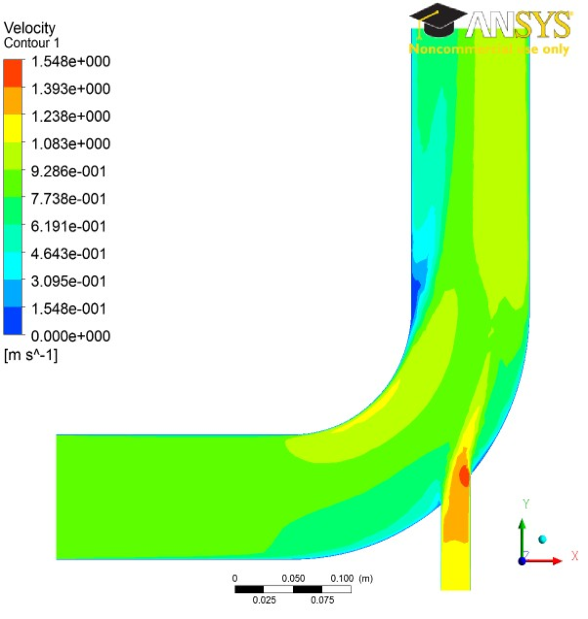
\includegraphics{background/5e1-1.pdf}
	\caption{Velocity distribution on the mid-plane for an inlet velocity for case 1.}
	\label{veldis}
\end{figure}
%%%%%%%%%%%%%%%%%%%%%%%%%%%%%%%%%%%%%%%%

The figure and caption should be centred. The figure numbering starts at 1 at the beginning of each chapter. The caption should provide a brief description of what is being shown. The figure should appear in the document after it is referred to in the text. No figure should be included which is not referred to in the text. Ensure that the size and resolution of images imported from software are sufficient to read any text.

\section{Tables}
Tables are an important way of displaying your results; Table \ref{tab:treatments} is a sample table, adapted from the Master/Doctoral Thesis template at \url{http://www.latextemplates.com/cat/theses}, which was generated with this code:

{\footnotesize
	\begin{verbatim}
\begin{table}[b]
\caption{The effects of treatments X and Y on the four groups studied.}
\label{tab:treatments}
\centering
\begin{tabular}{l l l}
\toprule
\textbf{Groups} & \textbf{Treatment X} & \textbf{Treatment Y} \\\midrule
1 & 0.2 & 0.8\\
2 & 0.17 & 0.7\\
3 & 0.24 & 0.75\\
4 & 0.68 & 0.3\\
\bottomrule\\
\end{tabular}
\end{table}
	\end{verbatim}
}

\begin{table}[b]
	\caption{The effects of treatments X and Y on the four groups studied.}
	\label{tab:treatments}
	\centering
	\begin{tabular}{l l l}
		\toprule
		\textbf{Groups} & \textbf{Treatment X} & \textbf{Treatment Y} \\
		\midrule
		1               & 0.2                  & 0.8                  \\
		2               & 0.17                 & 0.7                  \\
		3               & 0.24                 & 0.75                 \\
		4               & 0.68                 & 0.3                  \\
		\bottomrule\\
	\end{tabular}
\end{table}

Tables are numbered in the same way as figures. Typically tables also have a short caption, but this is not universally true. The number and caption appear above the table, not below as with figures. Again, no table should appear in the report which has not been referred to in the text. Tables should come after they are discussed in the text. The exact formatting of the table depends somewhat on the content of the table, but in general, the text in the table should be the same font and size as the main text. 

\section{Equations}
All equations should be numbered sequentially. Do not restart the numbering at the beginning of each chapter. Unlike figures and tables, you may not need to refer to every equation in the text. You should take care to format equations properly. Do no simply try to use plain text. Use the equation layout facilities. An example of how equations should appear is shown in Equation \ref{sampleequation}. Here is the code for it:

{\footnotesize
	\begin{verbatim}
\begin{equation}
\textrm{div}(\underline{u}) = \frac{\delta u}{\delta x} + \frac{\delta v}{\delta y} +
        \frac{\delta w}{\delta z} = 0
\label{sampleequation}
\end{equation} 
	\end{verbatim}
}

\begin{equation}
	\textrm{div}(\underline{u}) = \frac{\delta u}{\delta x} + \frac{\delta v}{\delta y} + \frac{\delta w}{\delta z} = 0
	\label{sampleequation}
\end{equation} 

\section{Referencing published work}
It is important to give appropriate credit to other people for the work that they have shared through publications. In fact, you must sign a declaration in your report stating that you understand the nature of plagiarism. As well as avoiding plagiarism, citing results or data from the literature can strengthen your argument, provide a favourable comparison for your results, or even demonstrate how superior your work is.

There are many styles to reference published work. For example, the parenthetical style (which is also called the Harvard style) uses the author and date of publication (e.g. ``Smith and Jones, 2001''). There is also the Vancouver (or the citation sequence) style, which is shown in this document. In the Vancouver style, the publications are cited using a bracket number which refers to the list in the References section at the end of the report. The references are listed in order that they are cited in the report. A variant is name sequence style in which the publications are referenced by number, but the list is arranged alphabetically. For example, the text might say: several studies have examined the sound field around tandem cylinders generated by flow\cite{fitzpatrick2003flow,finnegan2010experimental}, while other investigations have focused on the effect of an applied sound field on the flow\cite{hall2003vortex}. Papers from conference proceedings\cite{jordan2001array}, books\cite{paidoussis2010fluid} and technical reports\cite{reyes2007power,iea2011} can be dealt with in the same style.

The Vancouver style has the advantage that it is a little more compact in the text and does not distract from the flow of the sentence if there are a lot of citations. However, it has the disadvantage that it is not immediately clear to the reader what particular work has been referenced.

It actually does not matter which particular referencing style is used as long as three important considerations are observed:
\begin{itemize}
	\item the referencing style used throughout the document is consistent;
	\item all material used or discussed in the text is properly cited;
	\item nothing is included in the reference list that has not been cited.
\end{itemize}

This template has a suitable referencing style already set up -- you should use it and use the built-in BibTeX system to manage your references. See above for examples of how to cite a reference and look in the \texttt{sample.bib} file to see BibTeX references. Remember \href{http://scholar.google.com}{Google Scholar} and other search engines will give you BibTeX references for lots of academic publications. Otherwise, you can easily make up your own based on the examples in that file.

\chapter{Evaluation}
In this chapter, we concretely define our exact objectives for the experimentation aspect of this
project. We have implemented the system, which we use in our experimental apparatus and now wish to
carry out two case study based experiments. An inventory of our full experimental setup will be
given and we will close with the results of our case studies and a discussion of these results. What
we achieve, what we do not achieve and how our observations compare to published works.

\section{Objectives} \label{sec:eval_objectives}
The primary objective of our experimentation is to compare the performance of DRL-based AI agents that are trained
in Atari 2600 video game environments using 3 different DRL algorithms. We take a case study based
approach on the two games introduced in Section \ref{sec:games}; Space Invaders and Breakout. The
algorithms we use were introduced in Section \ref{sec:algos}, DQN, 2DQN and 3DQN. We compare the
effectiveness of these 3 algorithms using the metrics outlined in Section \ref{subsec:performance}.
\paragraph{}

The secondary outcomes of this experimentation are twofold. Firstly, it will test the flexibility
and stability of our system as we subject it to a range of games and algorithms. Secondly, it is our
hope that when we compare our results to those of published works, such as
(\citet{human,doubleq,dueling}), we can achieve similar results with our more limited resources.
\paragraph{}

\subsection{Performance Metrics} \label{subsec:performance}
In Section \ref{subsec:metrics} we introduced a choice selection of the more popular performance
metrics used in previously published works as well as in the current state of the art. For our
experiments, we gather the average game score and average frames survived for each set of evaluation
games. We also gather the average network loss for each training epoch to visualize the network's
learning performance over time. Finally, we record footage of the agent playing the game after
landmark stages of the training process: 500000, 750000 and 1 million steps. This is perhaps less of a
concrete, numerical metric but we believe that it gives context to the numbers and is to be used
more as a visual aid.

\section{Experimental Setup} \label{sec:setup}
We use Boole to run our system. Each job submitted to Boole consists of a
game-algorithm pair. This equates to 3 jobs/case study. Our system we have discussed in great detail
in Chapter \ref{ch:design}, however we will give a brief summary of how it will operate for our case
studies.

\begin{enumerate}
	\item The system is provided a game-algorithm pair on the command line when run.
	\item The agent will play the game for an epoch - 25,000 steps.
	\item After each step a gradient descent update is applied to the neural network, according to
	      the specified algorithm.
	\item After an epoch has completed, the agent plays the game 10 times. The scores and frames
	      survived are averaged for each game and saved to disk.
	\item Continue this loop until the 2 day limit on Boole is reached or the agent completes 20
	      epochs.
\end{enumerate}

Due to the constraints of time and resources discussed in Chapter \ref{ch:design}, we make the decision to scale down our hyper-parameters from the published values that we have taken inspiration from in (\citet{deepmind1,human,doubleq,dueling}). Our choice of scaling factor comes from our initial goal to train the agents for a minimum of 1 million steps. The standard in the aforementioned papers is to train for a minimum of 50 million steps, hence we scale our replay memory size and exploration rate decay $\epsilon_{decay}$ down by a factor of 50. We halve our training epoch length and reduce the target network update frequency $\tau$ to 25000 and 5000 respectively and cut the number of evaluation games from 30 to 10. A factor of 50 would be too extreme for these parameters.
\paragraph{}

We run the system on Boole, resubmitting jobs every 2 days from check-pointed positions thanks to
the systems state-saving functionality. The objective is to train each game-algorithm pair for a
minimum of 1 million steps. After this we can visualize our results by using the Python graphing
module, Matplotlib \cite{matplotlib} and perform our comparisons as stated previously.

\section{Experimental Results} \label{sec:results}
We present the final results of our experiments in tabular form in Table \ref{table:siscores} and
\ref{table:brscores}. These tables show the metrics collected for the evaluation run after 40 epochs of training. We present plots over time for each metric in Figures \ref{fig:score_plots}, \ref{fig:frames_plots} and \ref{fig:loss_plots}. \paragraph{}
\begin{table}[h]
	\centering
	\begin{tabular}{| c || c | c |}
		\hline
		\multicolumn{3}{|c|}{Space Invaders}                       \\
		\hline
		     & Final Average Score & Final Average Frames Survived \\
		\hline
		DQN  & 118                 & 2700                          \\
		\hline
		2DQN & 236                 & 2679                          \\
		\hline
		3DQN & 90.5                & 2176                          \\
		\hline
	\end{tabular}
	\caption{Space Invaders Final Results}
	\label{table:siscores}
\end{table}

\begin{table}[h]
	\centering
	\begin{tabular}{| c || c | c | c |}
		\hline
		\multicolumn{3}{|c|}{Breakout}                             \\
		\hline
		     & Final Average Score & Final Average Frames Survived \\
		\hline
		DQN  & 0                   & 0                             \\
		\hline
		2DQN & 0                   & 0                             \\
		\hline
		3DQN & 0.5                 & 976                           \\
		\hline
	\end{tabular}
	\caption{Breakout Final Results}
	\label{table:brscores}
\end{table}

In this Section we will give a comparison between DQN, 2DQN and 3DQN, based on the 3 different metrics outlined in Section \ref{subsec:performance}. Our immediate impression from the plots is that our agents did not perform as well as we would have hoped. The data for average score and average frames survived in both case studies is very noisy, showing no clear and obvious upward trends. 

\begin{figure}[H]
	\centering
	\begin{subfigure}{.3\textwidth}
		\centering
		\includegraphics[width=\linewidth]{score_si_dqn}
		\caption{Space Invaders DQN}
		\label{subfig:score_si_dqn}
	\end{subfigure}%
	\begin{subfigure}{.3\textwidth}
		\centering
		\includegraphics[width=\linewidth]{score_si_2dqn}
		\caption{Space Invaders 2DQN}
		\label{subfig:score_si_2dqn}
	\end{subfigure}%
	\begin{subfigure}{.3\textwidth}
		\centering
		\includegraphics[width=\linewidth]{score_si_3dqn}
		\caption{Space Invaders 3DQN}
		\label{subfig:score_si_3dqn}
	\end{subfigure}%
	\\
	\begin{subfigure}{.3\textwidth}
		\centering
		\includegraphics[width=\linewidth]{score_br_dqn}
		\caption{Breakout DQN}
		\label{subfig:score_br_dqn}
	\end{subfigure}%
	\begin{subfigure}{.3\textwidth}
		\centering
		\includegraphics[width=\linewidth]{score_br_2dqn}
		\caption{Breakout 2DQN}
		\label{subfig:score_br_2dqn}
	\end{subfigure}%
	\begin{subfigure}{.3\textwidth}
		\centering
		\includegraphics[width=\linewidth]{score_br_3dqn}
		\caption{Breakout 3DQN}
		\label{subfig:score_br_3dqn}
	\end{subfigure}
	\caption{Average Score Plots for Space Invaders \& Breakout}
	\label{fig:score_plots}
\end{figure}

\begin{figure}[H]
	\centering
	\begin{subfigure}{.3\textwidth}
		\centering
		\includegraphics[width=\linewidth]{frames_si_dqn}
		\caption{Space Invaders DQN}
		\label{subfig:frames_si_dqn}
	\end{subfigure}%
	\begin{subfigure}{.3\textwidth}
		\centering
		\includegraphics[width=\linewidth]{frames_si_2dqn}
		\caption{Space Invaders 2DQN}
		\label{subfig:frames_si_2dqn}
	\end{subfigure}%
	\begin{subfigure}{.3\textwidth}
		\centering
		\includegraphics[width=\linewidth]{frames_si_3dqn}
		\caption{Space Invaders 3DQN}
		\label{subfig:frames_si_3dqn}
	\end{subfigure}
	\\
	\begin{subfigure}{.3\textwidth}
		\centering
		\includegraphics[width=\linewidth]{frames_br_dqn}
		\caption{Breakout DQN}
		\label{subfig:frames_br_dqn}
	\end{subfigure}%
	\begin{subfigure}{.3\textwidth}
		\centering
		\includegraphics[width=\linewidth]{frames_br_2dqn}
		\caption{Breakout 2DQN}
		\label{subfig:frames_br_2dqn}
	\end{subfigure}
	\begin{subfigure}{.3\textwidth}
		\centering
		\includegraphics[width=\linewidth]{frames_br_3dqn}
		\caption{Breakout 3DQN}
		\label{subfig:frames_br_3dqn}
	\end{subfigure}
	\caption{Average Frames Survived Plots for Space Invaders \& Breakout}
	\label{fig:frames_plots}
\end{figure}

Our video footage further substantiates our claim. It is very obvious from watching the agent's gameplay that it makes very little progress in learning good game behaviour. The Space Invaders agent across all three algorithms fails to persistently dodge enemy bullets and track  the line of enemy ships. The Breakout agent does not recognize the ball at all and simply stays in the corner of the game screen, as the ball's first action is always to move to either corner. It does not learn to track the movement of the ball or learn the gameplay mechanic of returning the ball to hit the blocks. See Section \ref{sec:video_analysis} for further discussion on the accompanying video footage. \paragraph{}

After a similar amount of training time, the agents in (\citet{human,doubleq,dueling}) that we wish to compare against showed significantly more growth in average score. We compare the results of our DQN agent with (\citet{human}), our 2DQN agent with (\citet{doubleq}) and our 3DQN agent with (\citet{dueling}). \paragraph{}

\subsection{The High Average Loss of DQN} \label{sec:high_loss}
Before comparing our results, we will first explore the abnormally high average loss values for the DQN implementation of both case studies, as this was a problem unique to DQN. Loss was around the values of $10^{21}$ and $10^{13}$ in Space Invaders and Breakout respectively with very little reduction over time. This is indicative of an exploding gradient issue. Exploding gradient is caused when the gradient derivatives of the majority of nodes in a network are $>1$. As the Back Propagation algorithm is additive for each node in the graph, networks with many layers/nodes and individual gradients $>1$ can experience exploding gradients \paragraph{}

\begin{figure}[h]
	\centering
	\begin{subfigure}{.3\textwidth}
		\centering
		\includegraphics[width=\linewidth]{loss_si_dqn}
		\caption{Space Invaders DQN}
		\label{subfig:loss_si_dqn}
	\end{subfigure}%
	\begin{subfigure}{.3\textwidth}
		\centering
		\includegraphics[width=\linewidth]{loss_si_2dqn}
		\caption{Space Invaders 2DQN}
		\label{subfig:loss_si_2dqn}
	\end{subfigure}%
	\begin{subfigure}{.3\textwidth}
		\centering
		\includegraphics[width=\linewidth]{loss_si_3dqn}
		\caption{Space Invaders 3DQN}
		\label{subfig:loss_si_3dqn}
	\end{subfigure}%
	\\
	\begin{subfigure}{.3\textwidth}
		\centering
		\includegraphics[width=\linewidth]{loss_br_dqn}
		\caption{Breakout DQN}
		\label{subfig:loss_br_dqn}
	\end{subfigure}%
	\begin{subfigure}{.3\textwidth}
		\centering
		\includegraphics[width=\linewidth]{loss_br_2dqn}
		\caption{Breakout 2DQN}
		\label{subfig:loss_br_2dqn}
	\end{subfigure}%
	\begin{subfigure}{.3\textwidth}
		\centering
		\includegraphics[width=\linewidth]{loss_br_3dqn}
		\caption{Breakout 3DQN}
		\label{subfig:loss_br_3dqn}
	\end{subfigure}
	\caption{Average Loss Plots for Space Invaders \& Breakout. Note the exponential scale on the DQN y-axis}
	\label{fig:loss_plots}
\end{figure}

There are a number of standard techniques for overcoming exploding gradient problems in Deep Learning. Adding regularization terms imposes penalties on high weight updates. In Equation \ref{equ:regularization} we give the L2 or Ridge Regularization addition to a Mean Squared Error Loss Function as an example. $\lambda$ controls the  bias of the weight vector to lower values.

\begin{align}
	\label{equ:regularization}
	\sum^{n}_{i=1}(y_{i} - \sum^{p}_{j}x_{ij}w_{j})^{2} + \lambda \sum^{p}_jw^{2}_{j}
\end{align}

A second method is known as gradient clipping. In the same way that our reward clipping clamps the reward to the range $[-1, 1]$, we could do the same to individual gradients. \paragraph{}

The reason for our exploding gradient problem, we hypothesize, is that we did not use a target network in the implementation of this algorithm. As discussed in Section \ref{sec:improvements}, a target network can vastly improve the stability of the learning process by reducing the overestimation of Q-values and decreasing the likelihood of a diverging solution; exactly the dilemma in this case. In Figure \ref{fig:qvalues} we present a sample Space Invaders DQN and 2DQN (which uses a target network) Q-Value output for approximately the same state. We can see exactly how our network is grossly overestimating Q-values by comparing the two.

\begin{figure}[H]
	\centering
	$[4.0334538^{11}, 4.7766494^{11}, 3.7761424^{11}, 4.2299726^{11}, 4.0448184^{11}, 3.3483758^{11}]$ \\
	$[0.265942,  0.26520956,  0.26681688,  0.2608409, 0.26903862,  0.27122742]$
	\caption{Above: Output Q-values from the Space Invaders DQN implementation \\
		Below: Output Q-Values from the Space Invaders 2DQN implementation. Both values were taken at approximately the same state for a fair comparison.}
	\label{fig:qvalues}
\end{figure}

To further corroborate our hypothesis, (\citet{human}) conducted three further variants of their DQN experiment on five games:
\begin{itemize}
	\item With replay memory and without target network
	\item Without replay memory and with target network
	\item Without replay memory and without target network
\end{itemize}

The results of these are compared with the full implementation in Extended Data Table 3 of that paper. The agent had a 25\% drop in score in Breakout and 24\% drop in Space Invaders in the no target network test. \paragraph{}

\subsection{Comparison to Published Works}
As mentioned above, our results are well below those of published works and seem to show little to no correlation. For our DQN algorithm, we would expect Space Invaders to be reaching a score of 800-1000 as is accomplished by the agent in (\citet{human}). Although there are no progress graphs to show the learning progress of Space Invaders or Breakout for 2DQN in (\citet{doubleq}), they do however show graphs for Wizard of Wor and Asterix. These games show definite progress in the stages that our experiments finished at in terms of training time. There are no progress graphs in (\citet{dueling}), however it is a safe assumption to make that our results are not in line with theirs, as 3DQN is an improvement on DQN and 2DQN. \paragraph{}

After a thorough code review where no errors were found, we theorize that the problems lie with the decision we made to scale down the parameters of the experiments, not with our implementation of the system or algorithm logic. As discussed in Section \ref{sec:setup}, we down-scale several hyper-parameters from their published values to meet our requirements. \paragraph{}

We made an assumption that to facilitate our project constraints, it would be possible to shortcut the training of our agents by simply linearly scaling the scope of the original experiments. We postulate that the lost time spent exploring the environment due to the reduction of $\epsilon_{decay}$ is the cause of our agents' tendency to stay in one location, especially prevalent in the Breakout video footage. By losing out on the opportunity to take more random actions, the agent and the neural networks of our algorithms experience less states and are likely caught in a sub-optimal local minimum. If this is true, then further training after $\epsilon$ reaches $\epsilon_{min}$ would appear to be fruitless and a waste of time, as we would effectively be circling this local minimum. \paragraph{}

This could also be a factor in the reason why the average loss of our 2DQN and 3DQN algorithms are so low yet score performance is lacking - the agent is exploiting a very sub-optimal and narrow minded policy, thus it experiences the same states and the network outputs the same Q-Values over and over again. \paragraph{}

As published in the Extended Table 3 of (\citet{human}) that we referred to in Section \ref{sec:high_loss}, the scores of each of the five tested games were reduced dramatically when the replay memory was removed. We summarize the changes in Table \ref{table:replaymem}

\begin{table}[H]
	\centering
	\begin{tabular}{|c|c|c|}
		\hline
		Game           & With target network & Without target network \\
		\hline
		\hline
		Breakout       & 97\%                & 99\%                   \\
		\hline
		Space Invaders & 66\%                & 72\%                   \\
		\hline
	\end{tabular}
	\caption{Summary of the percentage reduction in score caused by the removal of replay memory.}
	\label{table:replaymem}
\end{table}

This highlights the importance of replay memory in the performance of the agents. We reduced the capacity of our replay memory significantly, hence we can estimate that this had a large bearing on the disappointing learning of our agents. Although we had a strict resource constraint imposed by Boole, as discussed in Section \ref{sec:replaymem}, these results cannot be ignored. In hindsight, we should have put further research into the exact limitations of our allocated physical memory with the Boole system administrator. \paragraph{}

To investigate whether or not parameterization was the crux of our problem, we requested access to a Boole partition that would allow our system to run for more than 2 days. Our initial estimates of achieving a minimum of 1 million frames for each case study was, in hindsight, conservative. We now know that this amount of training time is in fact feasible within the time frame of approximately one week for one algorithm. Our time constraints arise when we have to train 3 algorithms per case study. Thus, we decide to train Space Invaders and Breakout using the 3DQN algorithm with an updated set of hyper-parameters to see if the performance of our agents improve with less resource constraints. Our updated hyper-parameters are as follows:

\begin{itemize}
	\item Number of evaluation games from $10 \Rightarrow 30$
	\item Replay memory capacity from $20000 \Rightarrow 100000$
	\item $\epsilon_{decay}$ from $20000 \Rightarrow 100000$
\end{itemize}

We train these agents for 1 million steps each. The value of 100000 items for the replay memory capacity was found using an informal method of trial and error, whereby the job was submitted to Boole and if the capacity was too high the job would be kicked, we decrease the capacity and repeat. \paragraph{}

It was found that after 40 training epochs, the agents did not appear to have improved much over the original implementation. It is clear that the hyper-parameter values chosen by DeepMind were not randomly generated, and a good deal of optimization work was performed behind the scenes. (\citet{human}) confirm this, stating that all hyper-parameters were selected by performing an informal search on the games Pong, Breakout, Seaquest, Space Invaders and Beam Rider.

\subsection{Further Video Footage Analysis} \label{sec:video_analysis}
\subsubsection{Space Invaders}
The DQN agent shows high amount of movement between the edges of the game screen. It is not immediately apparent to us why it is doing this, there does not seem to be any strategy or reason to it. We consider it to be a result of the abnormally high average loss value discussed previously, the agent cannot determine the appropriate action to take in any given state so it's actions appear to us as random. The agent begins to show signs of dodging. If the agent is stationary and a bullet is oncoming, it may twitch slightly, but it is still sometimes too slow to react. As we will see in proceeding sections, the agent believes that shooting at all times is the best policy, and no concept of hunting is apparent. \paragraph{}

The 2DQN agent is quite deflating - it shows no signs of dodging or hunting. It remains stationary in the starting position and shoots for all actions, with negligible movement. It does not show any signs of dodging enemy bullets. \paragraph{}

The 3DQN agent shows movement similar to the DQN agent - seemingly random with no definite hunting pattern as it shoots randomly while moving across the screen. It displays some dodging, similar to the DQN agent there are cases where it is still to slow to react.

\subsubsection{Breakout}
A common theme among all Breakout agents is to move directly from the centre to a corner of the screen after each game reset. This is because the starting trajectory for the ball is always to either of the two corners, selected seemingly randomly. Thus, if the agent chooses the correct corner, it is likely to get a score of at least 1. It is likely that this has been caused by the small amount of exploration the agent accomplishes, as discussed in the previous section. As with the Space Invaders agents, there are no signs of hunting beyond moving directly to the corner.

\begin{figure}[h]
	\centering
	\includegraphics[width=\textwidth]{breakout_corners}
	\caption{The 2DQN Breakout agent moving directly to the right corner. On this occasion the ball's starting trajectory was to the right, and the agent managed to accumulate a few points.}
\end{figure}

\chapter{Conclusion}
In Section \ref{sec:sys_overview} we outlined three design goals for our system. In Section \ref{sec:eval_objectives} we outlined three goals for our experimentation. In this chapter we will restate those objectives and discuss whether or not we feel each goal was achieved. We will close with a discussion on what we felt we have learned from this project and the potential for future work.
\section{Goals Revisited}
\subsection{Design Goals}
We stated our design goals as follows:
\begin{enumerate}
	\item Support any game that the ALE does with no changes required in the code.
	\item Aid the implementation of additional algorithms for future developers.
	\item Provide a suite of useful research tools.
\end{enumerate}
It is our opinion that all of our design goals were achieved. Our system will work with all games that the ALE supports. We have aided the implementation of future algorithms by providing the \texttt{NN} base class, explained in Section \ref{sec:sys_overview}. The system comes equipped with various tools outlined in Section \ref{sec:sys_overview} - in our own experimentation we made use of all of these features regularly.

\subsection{Experimentation Goals}
We stated our experimentation goals as follows:
\begin{enumerate}
	\item Compare the performance of DRL-based AI agents trained in Atari 2600 video game environments using three state of the art DRL algorithms.
	\item Test the flexibility and rigour of our system.
	\item Achieve comparable results to that of published works.
\end{enumerate}
We feel that we have achieved our first and second experimentation goals and fell short of our third goal. \paragraph{}

Through our case study experiments, we have successfully compared the performance of two AI agents in the Space Invaders and Breakout Atari 2600 video game environments. We have gathered and presented the results of both case studies in Section \ref{sec:results}. \paragraph{}

The flexibility and stability of our system have been thoroughly tested. We have smoothly applied our implemented algorithms on two different games with no code changes. As mentioned in Section \ref{sec:setup}, the system was run for days on end, resulting in no crashes thus testifying to it's stability. \paragraph{}

Finally, our third goal was to attempt to achieve similar or comparable results to that of published works in (\citet{human,doubleq,dueling}). We have deemed that we have failed in this goal, owing primarily to the constraints of time and resources. Published works have trained their networks for much longer than our own - up to 50 million frames. Thus the resolution of their results is much broader. We have plotted our results over 40 epochs, where we treat an epoch as 25000 weight updates, (\citet{human}) have plotted their graphs to 200 epochs, where they treat an epoch as 50000 updates. Each of the aforementioned papers publish their final results only in tabular format. Thus it is difficult and would likely prove inaccurate to draw comparisons with their final results. \paragraph{}

In terms of resources, we have mentioned previously in Chapter \ref{ch:design} that much of our implementation such as training time, epoch duration and replay memory size are scaled down to suit our time and resource capabilities. It is likely that these actions negatively impacted our results - however they were a necessity.

\subsection{Project Goals}
We stated our overall project goals as follows:

\begin{enumerate}
	\item Investigate the current state of the art of RL for video games.
	\item Build a system to evaluate the performance of three state of the art DRL algorithms by collecting a series of metrics while applying each algorithm to a selection of Atari 2600 video games. 
	\item Compare and contrast the three algorithms by performing evaluation experiments. Investigate the game scores, survival times and model losses
\end{enumerate}

As we will discuss in Section \ref{sec:learning}, we have gained a significant amount of knowledge in the foundations of RL and RL in video games through the background research. The full accomplishment of our design goals allows us to conclude that the second project goal has been fulfilled - a fully working system has been built to evaluate the performance of DRL-based AI agents in Atari 2600 video games. Finally, although the results of our experimentation were lack-lustre, we did conduct a comparison of the three algorithms; DQN, 2DQN and 3DQN and sufficiently explained our opinions as to why the results were not as expected. Overall, we feel that the project was generally successful with potential for future work, which will be discussed in Section \ref{sec:future_work}.

\section{Learning Outcomes} \label{sec:learning}
I have learned much throughout the duration of this project. I now have a solid foundation of the theory of RL and a broad understanding and an appreciation for the relatively new field of DRL; it's landmark achievements, current state of the art, potential future endeavours and the software platforms used in it's research. From the case study experiments, I have have become familiar with the experimental approach for comparative studies. Lastly, I have increased my confidence and skill in designing and implementing a project of significant scale.

\section{Future Work} \label{sec:future_work}
There are a number of avenues that a future user of our system could explore. An obvious addition would be to implement different algorithms than those chosen in our experimentation. Of particular interest to us, we would recommend DQN with a target network, for the reasons discussed in Section \ref{sec:results}, A3C and any new state of the art algorithms that appear in the future. \paragraph{}

One interesting study would be to investigate potential efficiency improvements in the system. We would recommend exploring the feasibility of parallelization of the system, so that the network training could be distributed across multiple machines. This investigation would go hand-in-hand with an A3C algorithm implementation, as it is parallel by definition. This would be a worthwhile investigation, as it could aid in reducing the time constraint on network training that plagued this project throughout. It would be a significant technical undertaking, as it would require a third-party to become very familiar with a system that they are new to and did not build themselves. \paragraph{}

To further test the portability of our system, we would be interested to know if the range of environments could be extended to other platforms apart from the Atari 2600. Consoles such as the Gameboy \cite{gameboy} are similar to the Atari 2600 in terms of low-resolution graphics by today's standard, but provide enough of an improvement on the Atari 2600 to warrant investigation. The application of DRL algorithms to Gameboy video games is yet an unpublished field. The closest application that we could find was a system called Piglet \cite{piglet}, which uses other non-DRL techniques to produce AI agents.

\bibliographystyle{unsrtnat}
\bibliography{bibs/sample}
\appendix
\renewcommand{\thechapter}{A\arabic{chapter}}
\chapter{Appendix}
\section{ALE Supported Atari 2600 Games} \label{app:ALE_Games}
\begin{center}
    \begin{longtable}{ |c||c|c||c| }
        \hline
        ALE Format       & Game Title      & ALE Format         & Game Title        \\ [0.5ex]
        \hline
        \hline
        air\_raid        & Air Raid        & alien              & Alien             \\
        \hline
        amidar           & Amidar          & assault            & Assault           \\
        \hline
        asterix          & Asterix         & asteroids          & Asteroids         \\
        \hline
        atlantis         & Atlantis        & bank\_heist        & Bank Heist        \\
        \hline
        battle\_zone     & Battle Zone     & beam\_rider        & Beam Rider        \\
        \hline
        berzerk          & Berzerk         & bowling            & Bowling           \\
        \hline
        boxing           & Boxing          & breakout           & Breakout          \\
        \hline
        carnival         & Carnival        & centipede          & Centipede         \\
        \hline
        chopper\_command & Chopper Command & crazy\_climber     & Crazy Climber     \\
        \hline
        defender         & Defender        & demon\_attack      & Demon Attack      \\
        \hline
        double\_dunk     & Double Dunk     & elevator\_action   & Elevator Action   \\
        \hline
        enduro           & Enduro          & fishing\_derby     & Fishing Derby     \\
        \hline
        freeway          & Freeway         & frostbite          & Frostbite         \\
        \hline
        gopher           & Gopher          & gravitar           & Gravitar          \\
        \hline
        hero             & Hero            & ice\_hockey        & Ice Hockey        \\
        \hline
        jamesbond        & Jamesbond       & journey\_escape    & Journey Escape    \\
        \hline
        kangaroo         & Kangaroo        & krull              & Krull             \\
        \hline
        kung\_fu\_master & Kung Fu Master  & montezuma\_revenge & Montezuma Revenge \\
        \hline
        ms\_pacman       & Ms Pacman       & name\_this\_game   & Name This Game    \\
        \hline
        phoenix          & Phoenix         & pitfall            & Pitfall           \\
        \hline
        pong             & Pong            & pooyan             & Pooyan            \\
        \hline
        private\_eye     & Private Eye     & qbert              & Qbert             \\
        \hline
        riverraid        & Riverraid       & road\_runner       & Road Runner       \\
        \hline
        robotank         & Robotank        & seaquest           & Seaquest          \\
        \hline
        skiing           & Skiing          & solaris            & Solaris           \\
        \hline
        space\_invaders  & Space Invaders  & star\_gunner       & Star Gunner       \\
        \hline
        tennis           & Tennis          & time\_pilot        & Time Pilot        \\
        \hline
        tutankham        & Tutankham       & up\_n\_down        & Up N Down         \\
        \hline
        venture          & Venture         & video\_pinball     & Video Pinball     \\
        \hline
        wizard\_of\_wor  & Wizard Of Wor   & yars\_revenge      & Yars Revenge      \\
        \hline
        zaxxon           & Zaxxon                                                   \\
        \hline
    \end{longtable}
\end{center}

\section{Experimentation Hyper-Parameters} \label{app:hparams}
\begin{center}
    \begin{tabular}{||c|c|c||}
    \hline
    Hyper-parameter  & Value & Description \\ [0.5ex]
    \hline
    \hline
    minibatch size & 32 & Size of batch to sample from replay memory. \\
    \hline
    replay memory size & 20000 & \\
    \hline
    action repeat freq. & 3/4 & Number of frames to repeat the predicted action. \\
    \hline
    $\tau$, target network update freq.  & 5000  & Steps before updating target network weights. \\
    \hline
    $\epsilon_{max}$ initial exploration & 1.0   & Initial prob. of taking a random action. \\
    \hline
    $\epsilon_{min}$ final exploration & 0.1 & Final minimum prob. of taking a random action. \\
    \hline
    $\epsilon_{decay}$, exploration decay & 20000 & Number of steps to decay $\epsilon$ over. \\
    \hline
    $\gamma$, discount factor & 0.99 & Q-Learning discount factor. \\
    \hline
    $\alpha$, learning rate & 0.00025 & Neural network learning rate. \\
    \hline
\end{tabular}
\end{center}

These hyper-parameters were chosen with influence from (\citet{human}). They have been scaled down from those values to suit our requirements.



\end{document}